\documentclass[../main.tex]{subfiles}

\begin{document}
    \chapter{Related Work}\label{chap:related}

    In this chapter, we describe the domain adaptation problem in Section~\ref{sec:domainadapt}, highlighting the main challenges of the field.
    Then, in Section~\ref{sec:related-word} we review previous literature and we describe the most recent state-of-the-art approaches.
 
    \section{Domain Adaptation}\label{sec:domainadapt}

    In the following, we will restrict our discussion of ML algorithms to the subset of supervised learning, represented by algorithms that learns
    a function $y = f(x; \theta)$ mapping an input vector $x$ to an output vector $y$ parameterized by $\theta$.

    \paragraph{Introduction}
    Given a set of data $x$ and their associated value $y$, supervised machine learning algorithms aim at modeling their functional relation $y = f(x)$
    by minimizing the model's errors. The loss function $L(y, \hat{y}; \theta)$ evaluates the difference between the ground truth $y$ and the predicted $\hat{y}$
    on the basis of the model parameter $\theta$. The main challenge in this task is the reduction of the generalization error: the optimized model should not only
    be able to describe the available training data but it should also make reliable predictions on new test data not available at training time.

    \paragraph{The i.i.d.\ assumption}
    A typical assumption done in machine learning settings is that the \textit{training set}
    $( X_{train}, Y_{train} )$ (the sample used to minimize $L$) and the \textit{test set} $( X_{test}, Y_{test} )$
    (the sample used to evaluate generalization) are \textbf{i.i.d.}, namely independent and identically distributed. That is, each sample
    is independently drawn from the same underlying distribution $P(X, Y)$. The fact that samples are drawn independently is what allows us to write the loss function
    as a summation of a per-sample defined error function:
    $$ L_{sample}(y, \hat{y}; \theta) = \frac{1}{N} \sum_{i = 1}^{N} L(y_{i}, \hat{y_{i}}; \theta) $$
    The majority of learning algorithms operate under this assumption, which is usually a fairly good
    approximation. But there are cases in which this assumption does not hold, and this causes a significant drop between
    training and test performance.

    \paragraph{Motivation}
    Domain Adaptation~\cite{domain-adaptation-review} consists in the design of algorithms that work even when the i.i.d.\
    assumption does not hold~\footnote{Note that the assumption that samples are drawn independently is still valid.},
    i.e.\ when the distribution from which training samples are drawn is different from the one at test time.
    Domain adaptation has a slightly different terminology w.r.t.\ classical ML\@. In particular, the training distribution
    is called the \textit{source domain} $D_{S} \sim P_{s}(X, Y)$, while the test distribution is called the
    \textit{target domain} $D_{T} \sim P_{t}(X, Y)$.
    Typically, we assume that the source data is abundant and labeled, while the target data is either not or only partially labeled. \\
    The setting with no annotations available for the target is known as unsupervised D.A. While if the target is partially labeled we are
    in the semi-supervised setting.
    This thesis work in particular focuses exclusively on the (harder) unsupervised setting.
    
    \paragraph{Object Recognition}
    In the context of object recognition, the domain shift can be very large and it can have a variety
    of different causes, which can also interact between each other in nonlinear ways. Factors such as background, lighting
    condition, resolution, translation, scale and rotation, all contribute to the shift in distribution between source and target.
    The goal of an object recognition system is twofold. Firstly, it is to find the factors that explain variation the data.
    Secondly, it is to disentangle the factors that are specific to one domain, e.g.\ the background, from the factors that are shared across
    domains, e.g.\ the objects themselves.
    A human is capable of performing this task accurately and reliably in a matter of milliseconds, but it has been beyond the
    reach of computer vision and machine learning algorithms for decades. We hope that the method presented in this thesis work
    provides a step in the right direction in order to improve object recognition systems and to provide promising directions
    of future research.
    
    \begin{figure}[h!]
        \centering

        \begin{subfigure}{\linewidth}
        	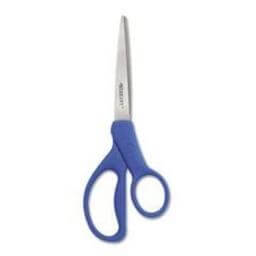
\includegraphics[width=.3\linewidth]{img/amazon-scissor.png}\label{fig:amazon-scissor}\hfill
        	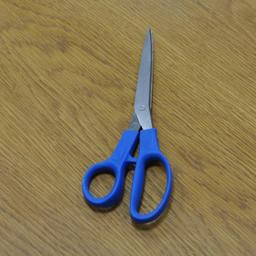
\includegraphics[width=.3\linewidth]{img/dslr-scissor.png}\label{fig:dslr-scissor}\hfill
            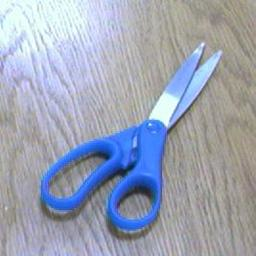
\includegraphics[width=.3\linewidth]{img/webcam-scissor.png}\label{fig:webcam-scissor}
        \end{subfigure}

        \caption{Examples of visual domain shift. The shift between the left and center images is clearly
            due to the background. The shift between the center and right images is due to resolution. In fact, the center
            image was taken with a high-resolution camera, while the right image was taken with a webcam.}\label{fig:domain-shift-office}
	   \end{figure}

    \paragraph{Domain Adaptation}
    In ML, the joint distribution between data and labels $P(X, Y)$ is unknown. In domain adaptation,
    we call the joint distribution of the source domain $ P_{s}(X, Y) $, while $ P_{t}(X, Y) $ is the joint distribution of
    the target domain. The i.i.d.\ assumption consists in a assuming that $ P_{s}(X, Y) = P_{t}(X, Y) = P(X, Y) $.
    In Domain Adaptation instead, we have $ P_{s}(X, Y) \neq P_{t}(X, Y) $. We can visualize what the implications
    of this fact are in figure~\ref{fig:AD-tsne}.
    \newline
    The source data is drawn i.i.d.\ from the source distribution, while the target data is drawn i.i.d.\ from the target marginal
    distribution over $X$:
    \begin{align*}
        S = {\{(x_{i}, y_{i})\}}_{i=1}^{N} \sim {(D_{S})}^{N} \\
        T = {\{(x_{i})\}}_{i=1}^{M} \sim {(D_{T}^{X})}^{M}
    \end{align*}
    The goal is to build a classifier $f : X \rightarrow Y$ capable of making correct predictions about the target labels $Y_{t}$:
    $$ \theta^{\star} = \max_{\theta} P(Y_{t} = \hat{Y_{t}} | X_{t} ; \theta) $$
    Where $\hat{Y_{t}} = f(X_{t})$ are the labels predicted by the classifier and $Y_{t}$ are the true target labels, which we
    don't have access to.

    \begin{figure}
        \centering{}
    	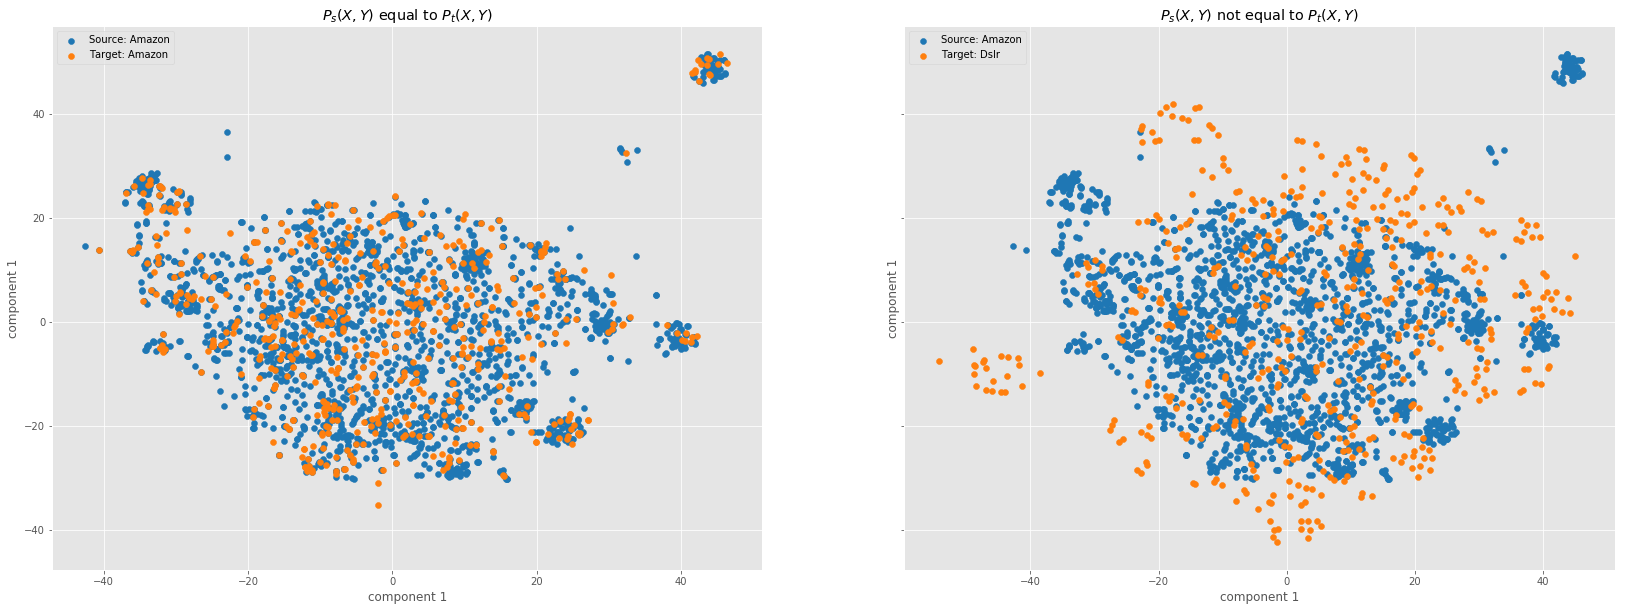
\includegraphics[width=\linewidth]{img/AD-alexnet-tsne.png}
        \caption{t-SNE~\cite{tsne} visualization of the features extracted from the Office dataset~\cite{office} using AlexNet~\cite{alexnet}.
        When the source and the target distribution are the same (left), a classifier trained on the source data generalizes very well to the target
        data. When the i.i.d.\ assumption does not hold (right), the model will generalize poorly.}\label{fig:AD-tsne}
	\end{figure}

    \section{Domain Adaptation approaches}\label{sec:related-word}
	Domain Adaptation is a fundamental problem in machine learning, and the need for techniques that works when
	$P_{s}(X, Y) \neq P_{t}(X, Y)$ is preminent in the majority of practical applications. In computer vision in particular,
	there is a large number of factors which can cause the domain shift: background, lighting conditions, resolution and scale,
	position and orientation of the object of interest and so on. Various approaches to address the domain adaptation problem
	have been proposed in the literature. In the following overview of the domain adaptation literature, we will use the same
	distinction of~\cite{DBLP:journals/corr/Csurka17} into shallow methods and the more recent deep methods, which employs
	deep learning models, in particular the deep convolutional networks described in Section~\ref{sec:deeplearning}.

    \subsection{Shallow Methods}
	In this context, shallow methods refers to those methods based on feature vector representations $\phi(X)$ extracted from
	the images with non-deep-learning methods.

	\paragraph{Instance Weighting}
	The earliest solutions to the domain adaptation problem go under the name
	of \textit{Instance Weighting} approaches.
	The basic idea is that of assigning a different weight to each source sample in the computation of the loss. The definition of the
	weight varies based on the assumptions one makes about the source and target distributions. One possible approach is assuming
	that the conditional distributions of the labels given the same observation are the same, but clearly the marginal distributions
	of the observations are different. Formally:
	$$ P_{s}(Y | X = x) = P_{t}(Y | X = x) \text{ with } P_{s}(X) \neq P_{t}(X) $$
	This assumption is called \textit{covariate shift} and it is explored in depth in~\cite{shimoidara2000}. To solve the covariate
	shift problem,~\cite{shimoidara2000} weights each training instance with $\frac{P_{t}(X)}{P_{s}(X)}$, that is, the weight is the
	ratio between the likelihood of being a target and a source sample.

	\paragraph{Feature Space Alignment}
	Another class of techniques try to align source features with the target ones. A very simple method in this class is
	Subspace Alignment (SA)~\cite{subspace-alignment}, where the alignment is made between the subspaces obtained by PCA reduction:
	$$ P_{s} = PCA(X_{s}, d) \qquad P_{t} = PCA(X_{t}, d) $$
	$$ X_{s}^{'} = X_{s}P_{s}P_{s}^{T}P_{t} \qquad X_{t}^{'} = X_{t} P_{t} $$
	And then $X_{s}^{'}$ and $X_{t}^{'}$ are used in place of $X_{s}$ and $X_{t}$.

	\paragraph{Feature Transformation through metric learning}
	Some domain adaptation approaches exploit metric learning solutions but in most of the cases they need labeled data both in the source
    and in the target domain. The only method that used this strategy in the unsupervised setting is DA-NBNN~\cite{da-nbnn}.
    Its main idea was to iteratively replace the most ambiguous
	source example of each class by the target example for which the classifier (Naive Bayes Nearest Neighbor (NBNN)) is the
	most confident for the given class. It does this by iteratively learning a metric of the relatedness between the source and
	target domains.

    \subsection{Deep methods}
	The expression deep methods refers to all those approaches which are based either on fixed features extracted from a deep learning
    model or on the design of a novel deep network architecture which encorporates elements to solve the domain adaptation problem.
    One method worth mentioning in this respect is the Domain Adversarial Neural Networks (DANN)~\cite{DANN}, which obtained state-of-the-art
    results on several benchmark datasets. It is called adversarial training because a part of the network is optimized in such a way
    to confuse another part of the network.

    \subsubsection{DANN}
      \begin{figure}[!ht]
          \centering{}
      	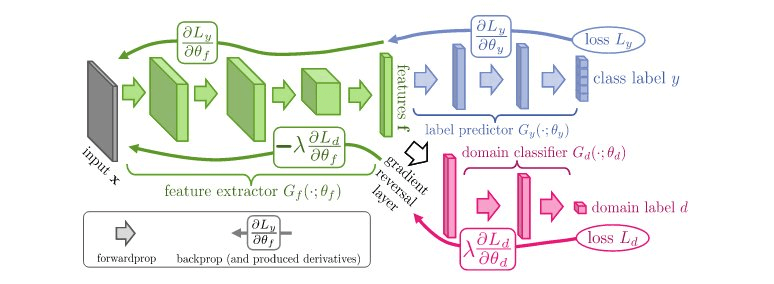
\includegraphics[width=\linewidth]{img/dann-architecture.png}
          \caption{DANN Architecture. Image taken from~\cite{DANN}.}\label{fig:dann-architecture}
  	  \end{figure}

    The network is composed of three parts:
    \begin{itemize}
        \item \textbf{feature extractor}: this part of the network is trained to simultaneously optimize two objetives: learn features
            that are discriminant for the source classification task, and at the same time learn domain invariant features, that is,
            features that would increase the classification error of a binary domain classifier.
        \item \textbf{image classifier}: this is the classifier that carries on the main image classification task.
        \item \textbf{domain classifier}: this is the binary classifier that carries on the domain classification task between source and
            target. It is the adversary of the feature extractor.
    \end{itemize}
    
    DANN is not a novel architecture per se. Instead, it can be thought of as a
    method to extend existing networks to perform domain adaptation. One feature
    of DANN worth mentioning is that it is application-agnostic, namely
    it is general enough that it can be applied to different areas, such as
    computer vision, natural language processing and speech recognition.
    This is different with respect to our method, which is designed specifically
    for computer vision applications.

\end{document}
